\documentclass[10pt]{amsart}
\usepackage[a4paper,margin=22mm]{geometry}
\usepackage[no-math]{fontspec}
\setmainfont{Latin Modern Roman}[SmallCapsFont={lmromancaps10-regular.otf}]
\usepackage{amsmath,amssymb,amsthm,mathtools,hyperref,graphicx,float}
\usepackage[shortlabels]{enumitem}
\emergencystretch=3em
\newtheorem{theo}{Theorem}[section]
\newtheorem{lemm}[theo]{Lemma}
\newtheorem{prop}[theo]{Proposition}
\newtheorem{coro}[theo]{Corollary}
\theoremstyle{definition}
\newtheorem{defi}[theo]{Definition}
\newtheorem{rema}[theo]{Remark}
\newtheorem{exam}[theo]{Example}
\newtheorem{nota}[theo]{Notation}
\providecommand{\ie}{i.e.\ }
\providecommand{\eg}{e.g.\ }
\providecommand{\etc}{etc.\ }
\DeclarePairedDelimiter\abs{\lvert}{\rvert} 
\DeclareMathOperator{\reg}{reg}
\DeclareMathOperator{\Tor}{Tor}
\DeclareMathOperator{\pol}{pol}


\newcommand{\NN}{{\mathbb N}}
\newcommand{\F}{\mathcal{F}}
\newcommand{\E}{\mathcal{E}}
\newcommand*{\mk}{\mkern -1mu}
\newcommand*{\Mk}{\mkern -2mu}
\newcommand*{\mK}{\mkern 1mu}
\newcommand*{\MK}{\mkern 2mu}

\hypersetup{urlcolor=purple, linkcolor=blue, citecolor=red}


\newcommand*{\romanenumi}{\renewcommand*{\theenumi}{\roman{enumi}}}
\newcommand*{\Romanenumi}{\renewcommand*{\theenumi}{\Roman{enumi}}}
\newcommand*{\alphenumi}{\renewcommand*{\theenumi}{\alph{enumi}}}
\newcommand*{\Alphenumi}{\renewcommand*{\theenumi}{\Alph{enumi}}}
\title[Uniform regularity bounds from local graph data]{Uniform edge-ideal power regularity from deletion-monotone local bounds on a graph hierarchy}
\author{Arindam Banerjee}
\author{Selvi Kara Beyarslan}
\author{Huy T\`ai H\`a}
\date{Algebraic Combinatorics3(4)(2020),839–854; DOI10.5802/alco.119}
\hypersetup{hidelinks}
\begin{document}
\maketitle
\setcounter{section}{1}
\section{Preliminaries}\label{chapter2}

In this section, we collect notations and terminology used in the paper. For unexplained notions, we refer the reader to standard texts~\cite{BrHe, E, Harary, HH, MS, Stanley, V}.

%\begin{enonce*}[remark]{Graph Theory}
\subsection{Graph Theory} 
Throughout the paper, $G$ shall denote a finite simple graph with vertex set $V(G)$ and edge set $E(G)$. A subgraph $G'$ of $G$ is called \emph{induced} if for any two vertices $u,v$ in $G'$, $uv \in E(G') \Leftrightarrow uv \in E(G)$. For a subset $W \subseteq V(G)$, we shall denote by $G_W$ the induced subgraph of $G$ over the vertices in $W$, and denote by $G-W$ the induced subgraph of $G$ on $V(G) \setminus W$. When $W = \{w\}$ consists of a single vertex, we also write $G-w$ for $G-\{w\}$. The \emph{complement} of a graph $G$, denoted by $G^c$, is the graph on the same vertex set $V(G)$ in which $uv \in E(G^c) \Leftrightarrow uv \not\in E(G)$.
%\end{enonce*}


\begin{defi} Let $G$ be a graph.
\begin{enumerate}
\item\label{def2.1_1} A \emph{walk} in $G$ is a sequence of (not necessarily distinct) vertices $x_1,x_2, \dots, x_n$ such that $x_ix_{i+1}$ is an edge for all $i=1,2,\dots,n-1.$
\item\label{def2.1_2} A \emph{path} in $G$ is a walk whose vertices are distinct (except possibly the first and the last vertices).
\item\label{def2.1_3} A \emph{cycle} in $G$ is a closed path. A cycle consisting of $n$ distinct vertices is called an $n$-cycle and often denoted by $C_n.$
\item\label{def2.1_4} An \emph{anticycle} is the complement of a cycle.
\end{enumerate}
\end{defi}

A graph in which there is no induced cycle of length greater than 3 is called a \emph{chordal} graph. A graph whose complement is chordal is called a \emph{co-chordal} graph.

\begin{defi} Let $G$ be a graph.
\begin{enumerate}
\item\label{def2.2_1} A \emph{matching} in $G$ is a collection of disjoint edges. The \emph{matching number} of $G$, denoted by $\beta(G)$ is the maximum size of a matching in $G$.
\item\label{def2.2_2} An \emph{induced matching} in $G$ is a matching $C$ such that the induced subgraph of $G$ over the vertices in $C$ does not contain any edge other than those already in $C$. The \emph{induced matching number} of $G$, denoted by $\nu(G)$, is the maximum size of an induced matching in $G$.
\item\label{def2.2_3} A \emph{vertex cover} of $G$ is a collection of vertices in $G$ that contains at least one endpoint of every edge in $G.$
\end{enumerate}
\end{defi}
\setcounter{theo}{5}
\begin{nota} Let $G$ be a graph, let $u,v \in V(G)$, and let $e = xy \in E(G)$.
\begin{enumerate}
\item\label{nota2.6_1} The set of vertices incident to $u$, the \emph{neighborhood} of $u$, is denoted by $N_G(u)$. Set $N_G[u] = N_G(u) \cup \{u\}$.
\item\label{nota2.6_2} The set of vertices which are not in $e$ and incident to an endpoint of $e$, the \emph{neighborhood} of $e$, is denoted by $N_G(e)$. Set $N_G[e] = N_G(e) \cup e.$
\item\label{nota2.6_3} The \emph{degree} of $u$ is $\deg_G(u) = \big|N_G(u)\big|$. An edge is called a \emph{leaf} or a \emph{whisker} if any of its vertices has degree exactly 1.
\end{enumerate}
\end{nota}

We can naturally extend these notions to get $N_G(W)$, $N_G[W]$, $N_G(\E)$ and $N_G[\E]$ for a subset of the vertices $W \subseteq V(G)$ or a subset of the edges $\E \subseteq E(G)$. Particularly, $N_G(W)$ denotes the set of vertices which are not in $W$ and incident to a vertex in $W$, $N_G[W] = N_G(W) \cup W$, and $N_G(\E)$ is the set of vertices which are not in any of the edges in $\E$ and incident to an endpoint of an edge in $\E$, $N_G[\E] = N_G(\E) \cup (\cup_{e \in \E} e)$.


\subsection{Commutative Algebra} 
Let $G$ be a graph over the vertices $V(G)  = \{x_1, \dots, x_n\}$. By abusing notation, we shall identify the vertices of $G$ with the variables in a polynomial ring $S = k[x_1, \dots, x_n]$, where $k$ is field. Particularly, we shall use $uv$ to denote both the edge $uv$ in $G$ and the monomial $uv$ in $S$ (the choice would be obvious from the context).

\begin{defi} Let $G$ be a graph over the vertices $V(G) = \{x_1, \dots, x_n\}$. The \emph{edge ideal} of $G$ is defined to be
\[
I(G) =( xy  \mid  xy \in E(G)) \subseteq S.
\]

\end{defi}

Castelnuovo--Mumford regularity is \emph{the} invariant being investigated in this paper. We shall give a definition most suitable for our context (see, for example,~\cite[p. 168]{BrHe}).

\begin{defi}
Let $S$ be a standard graded polynomial ring over a field $k$. The \emph{regularity} of a finitely generated graded $S$-module $M$, written as $\reg M$, is given by
\[
\reg M := \max \{j-i|\Tor_{i} (M,k)_j \neq 0 \}.
\]

\end{defi}



The following simple bound is often used without references; it follows immediately from Hochster's formula~\cite[Theorem 5.1]{Hochster}.

\begin{lemm}\label{lem.indsubgraph}
Let $G$ be a graph and let $H$ be an induced subgraph of $G$. Then
\[
\reg I(H) \le \reg I(G).
\]
Particularly, for any vertex $v \in V(G)$, we have that $\reg I(G - v) \le \reg I(G).$
\end{lemm}

A standard use of short exact sequences yields the following result, which we shall also often use (see~\cite[Lemma 2.10]{DHS} and~\cite[Lemma 2.11]{Ba}).

\begin{lemm}\label{exact}
Let $I \subseteq S$ be a monomial ideal, and let $m$ be a monomial of degree $d$. Then
\[
\reg I \le \max\{ \reg (I : m) + d, \reg (I,m)\}.
\]
Moreover, if $m$ is a variable appearing in I, then $\reg I$ is \emph{equal} to one of the right-hand-side terms.
\end{lemm}

\begin{defi} Let $r \in \NN$. A graph $G$ is said to be \emph{locally of regularity $\le r$} if for every vertex $x \in V(G)$, we have $\reg (I(G):x) \le r$. A graph which is locally of regularity $\le 2$ is called \emph{locally linear}.
\end{defi}

\subsection{Auxiliary Results} 
We next recall a few results that are useful for our purpose.

We shall make use of the following characterization for edge ideals of graphs with linear resolutions. This characterization was first given in topological language by Wegner~\cite{Wegner} and later, independently, by Lyubeznik~\cite{L} and Fr\"oberg~\cite{Fr} in monomial ideals language.

\begin{theo}[\protect{See~\cite[Theorem 1]{{Fr}}}] \label{thm.regtwo}
Let $G$ be a graph. Then $\reg I(G) = 2$ if and only if $G$ is a co-chordal graph.
\end{theo}


In the study of powers of edge ideals, Banerjee developed the notion of even-connection and gave an important inductive inequality in~\cite{Ba}. This inductive method has proved to be quite powerful, which we shall make use of often.

\begin{theo}\label{thm.inductive}
For any graph $G$ and any $s\geq 1$, let the set of minimal monomial generators of $I(G)^s$ be $\{m_1,....,m_k\}$, then \[
\reg I(G)^{s+1} \leq \max \{ \reg (I(G)^{s+1} : m_l)+2s, 1\leq l \leq k, \reg I(G)^s\}.
\]

\end{theo}

\begin{rema}
Any minimal generator of $I(G)^s$ is the product of $s$ edges in $G$ and, vice-versa, for any $s$ edges $e_1, \ldots, e_s$ of $G$ the $s$-fold product $e_1 \cdots e_s$ is a minimal generator of $I(G)^s$. Note that a minimal generator of $I(G)^s$ may come from different choices of $s$ edges in $G$. 
\end{rema}

 The ideal $(I(G)^{s+1}: m)$ in Theorem~\ref{thm.inductive} and its generators are understood via the following notion of even-connection.

\begin{defi}\label{even_connected} Let $G=(V,E)$ be a graph. Two vertices $u$ and $v$ ($u$ may be the same as $v$) are
said to be even-connected with respect to an $s$-fold product $e_1\cdots e_s$ where $e_i$'s are edges of $G$, not necessarily distinct,
if there is a path $p_0,p_1,\ldots, p_{2k+1}$, $k\geq 1$, in $G$ such that:
\begin{enumerate}
 \item\label{def2.15_1} $p_0=u,p_{2k+1}=v.$
 \item\label{def2.15_2} For all $0 \leq l \leq k-1,$ $p_{2l+1}p_{2l+2}=e_i$ for some $i$.
 \item\label{def2.15_3} For all $i$, $\big|\{l \geq 0 \mid p_{2l+1}p_{2l+2}=e_i \}\big| \le \big|\{j \mid e_j=e_i\}\big|$.
\end{enumerate}
\end{defi}

It turns out that $(I(G)^{s+1} : m)$ is generated by monomials in degree 2.

\begin{theo}[\protect{\cite[Theorem 6.1 and Theorem 6.7]{Ba}}] \label{even_connec_equivalent}
Let $G$ be a graph with edge ideal
$I$, and let $s \geq 1$ be an integer. Let $m$ be a minimal generator of $I^s$.
Then $(I^{s+1} : m)$ is minimally generated by monomials of degree 2, and $uv$ ($u$ and $v$ may
be the same) is a minimal generator of $(I^{s+1} : m )$ if and only if either $\{u, v\} \in E(G) $ or $u$ and $v$ are even-connected with respect to $m$.
 \end{theo}

Thanks to Theorems~\ref{thm.inductive} and~\ref{even_connec_equivalent}, much of our work is to understand colon ideals of the form $I(G)^{s+1}:m$, when $m$ is a minimal generator of $I^s$. Our technique is to use \emph{polarization} to bring such an ideal to a squarefree monomial ideal and to look at its corresponding graph. Note that the regularity does not change in passing to the polarization; see, for example,~\cite[Corollary 1.6.3]{HH}.

\begin{defi}\label{def.polarization}
\index{polarization}
Let $I \subseteq S = k[x_1, \ldots, x_n]$ be a monomial ideal.
For each $i = 1, \ldots, n$ let $a_i$ be the maximum power of $x_i$ appearing in the monomial generators of $I$. The \emph{polarization} of $I$, denoted by $I^{\pol}$, is constructed as follows.
\begin{itemize}
\item Let $S^{\pol} = k[x_{11}, \ldots, x_{1a_1}, \ldots, x_{n1}, \ldots, x_{na_n}]$.
\item The ideal $I^{\pol}$ is generated by monomials in $S^{\pol}$ that are obtained from generators of $I$ under the following substitution, for each $(\gamma_1, \ldots, \gamma_n) \le (a_1, \dots, a_n)$,
\[
x_1^{\gamma_1} \cdots x_n^{\gamma_n} \longrightarrow x_{11} \cdots x_{1\gamma_1} \cdots x_{n1} \cdots x_{n\gamma_n}.
\]

\end{itemize}
\end{defi}

\begin{rema} \label{rmk.G'}
	In the polarization process, we can identify $x_{11}, \ldots, x_{n1}$ with $x_1, \ldots, x_n$. Let $G'$ be the graph corresponding to the polarization of $I^{s+1}:m$, where $m$ is a minimal generator of $I^s$. By Theorem~\ref{even_connec_equivalent}, $G'$ is obtained from $G$ by adding edges $uv$, where $u,v \in V(G)$ are even-connected with respect to $m$ in $G$, and \emph{whiskers} $uu'$, where $u \in V(G)$ is even-connected to itself with respect to $m$ in $G$ and $u'$ is a new vertex.
\end{rema}



\section{General Upper Bounds for Regularity Function} \label{chapter3}

The aim of this section is to give a weaker general upper bound for $\reg I(G)^s$ than that of Conjecture A.

The heart of many studies on regularity of powers of edge ideals is to understand the colon ideal $J = I(G)^s : e_1 \cdots e_{s-1}$ in making use of Banerjee's inductive method, Theorem~\ref{thm.inductive}. We start by examining a local property for $J$.

\begin{lemm} \label{lem.induction}
Let $G$ be a graph with edge ideal $I$ and let $s \in \NN$. Let $e_1, \dots, e_{s-1} \in E(G)$, $J = I^s : e_1 \cdots e_{s-1}$, and let $G'$ be the graph associated to the polarization of $J$. Let $w \in V(G)$.
\begin{enumerate}
\item\label{lemma3.1_1} If $e_1$ is a leaf of $G$ then $J = I^{s-1} : e_2 \cdots e_{s-1}$.
\item\label{lemma3.1_2} Suppose that $w \not\in N_G[\{e_1, \dots, e_{s-1}\}]$. Then
\[
J:w = I(G - N_G[w])^s : e_1 \cdots e_{s-1} + (u ~\big|~ u \in N_G[w]).
\]

\item\label{lemma3.1_3} Suppose that $w \in N_G[e_1]$. Then
\[
J:w = (I(G - N_{G'}[w])^t : f_1 \cdots f_{t-1}) + (u ~\big|~ u \in N_{G'}(w))
\]
for some $t \le s$, and a subcollection $\{f_1, \dots, f_{t-1}\}$ of $\{e_2, \dots, e_{s-1}\}$. Moreover, in this case, the graph associated to the polarization of $I(G-N_{G'}[w])^t : f_1 \cdots f_{t-1}$ is an induced subgraph of that associated to the polarization of $I(G-N_G[w])^t : f_1 \cdots f_{t-1}$.
\end{enumerate}
\end{lemm}

\begin{proof} \eqref{lemma3.1_1}~It follows from Theorem~\ref{even_connec_equivalent} that $J$ is obtained by adding to $I$ quadratic generators $uv$, where $u$ and $v$ are even-connected in $G$ with respect to $e_1 \cdots e_{s-1}$. If $e_1$ is an isolated edge then clearly, by definition, the even-connected path between $u$ and $v$ does not contain $e_1$. Thus, $uv \in I^{s-1} : e_2 \cdots e_{s-1}$ and~\eqref{lemma3.1_1} is proved.

\eqref{lemma3.1_2}~It can be seen that if $w \not\in N_G[\{e_1, \dots, e_{s-1}\}]$ then $w$ is not in any even-connected path with respect to $e_1 \cdots e_{s-1}$. Thus, even-connected paths with respect to $e_1 \cdots e_{s-1}$ between two vertices that are not in $N_G[w]$ are even-connected path with respect to $e_1 \cdots e_{s-1}$ in $G - N_G[w]$. Furthermore, any edge $uv \in J$, for which $u \in N_G[w]$ (similarly if $v \in N_G[w]$), would be divisible by $u \in J:w$ and, thus, subsumed into the ideal $(u ~\big|~ u \in N_G[w])$. Therefore,~\eqref{lemma3.1_2} follows.

\begin{figure}[htb]
 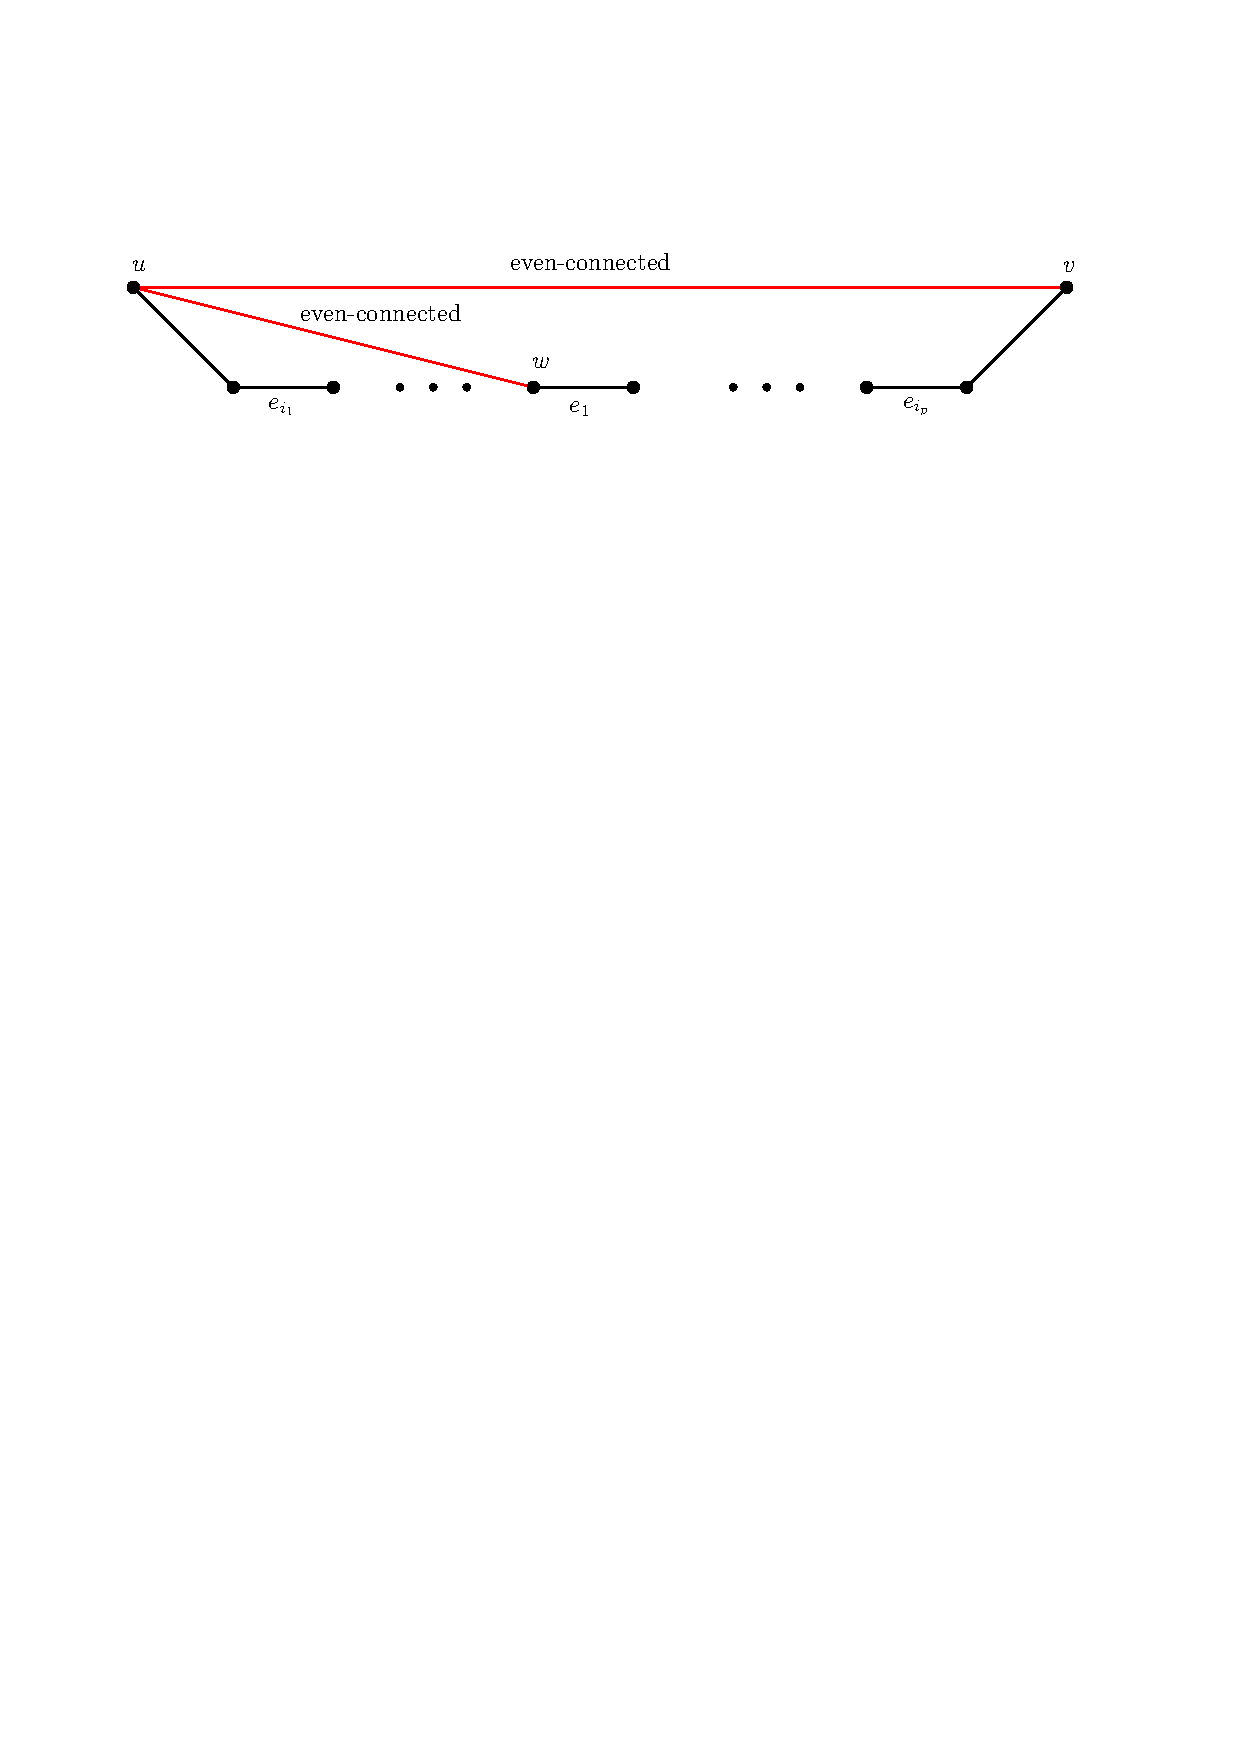
\includegraphics[width=0.9\linewidth]{figures/even1.pdf}
 \caption{When $w \in e_1$}
 \label{fig:even1}
\end{figure}

\begin{figure}[htb]
 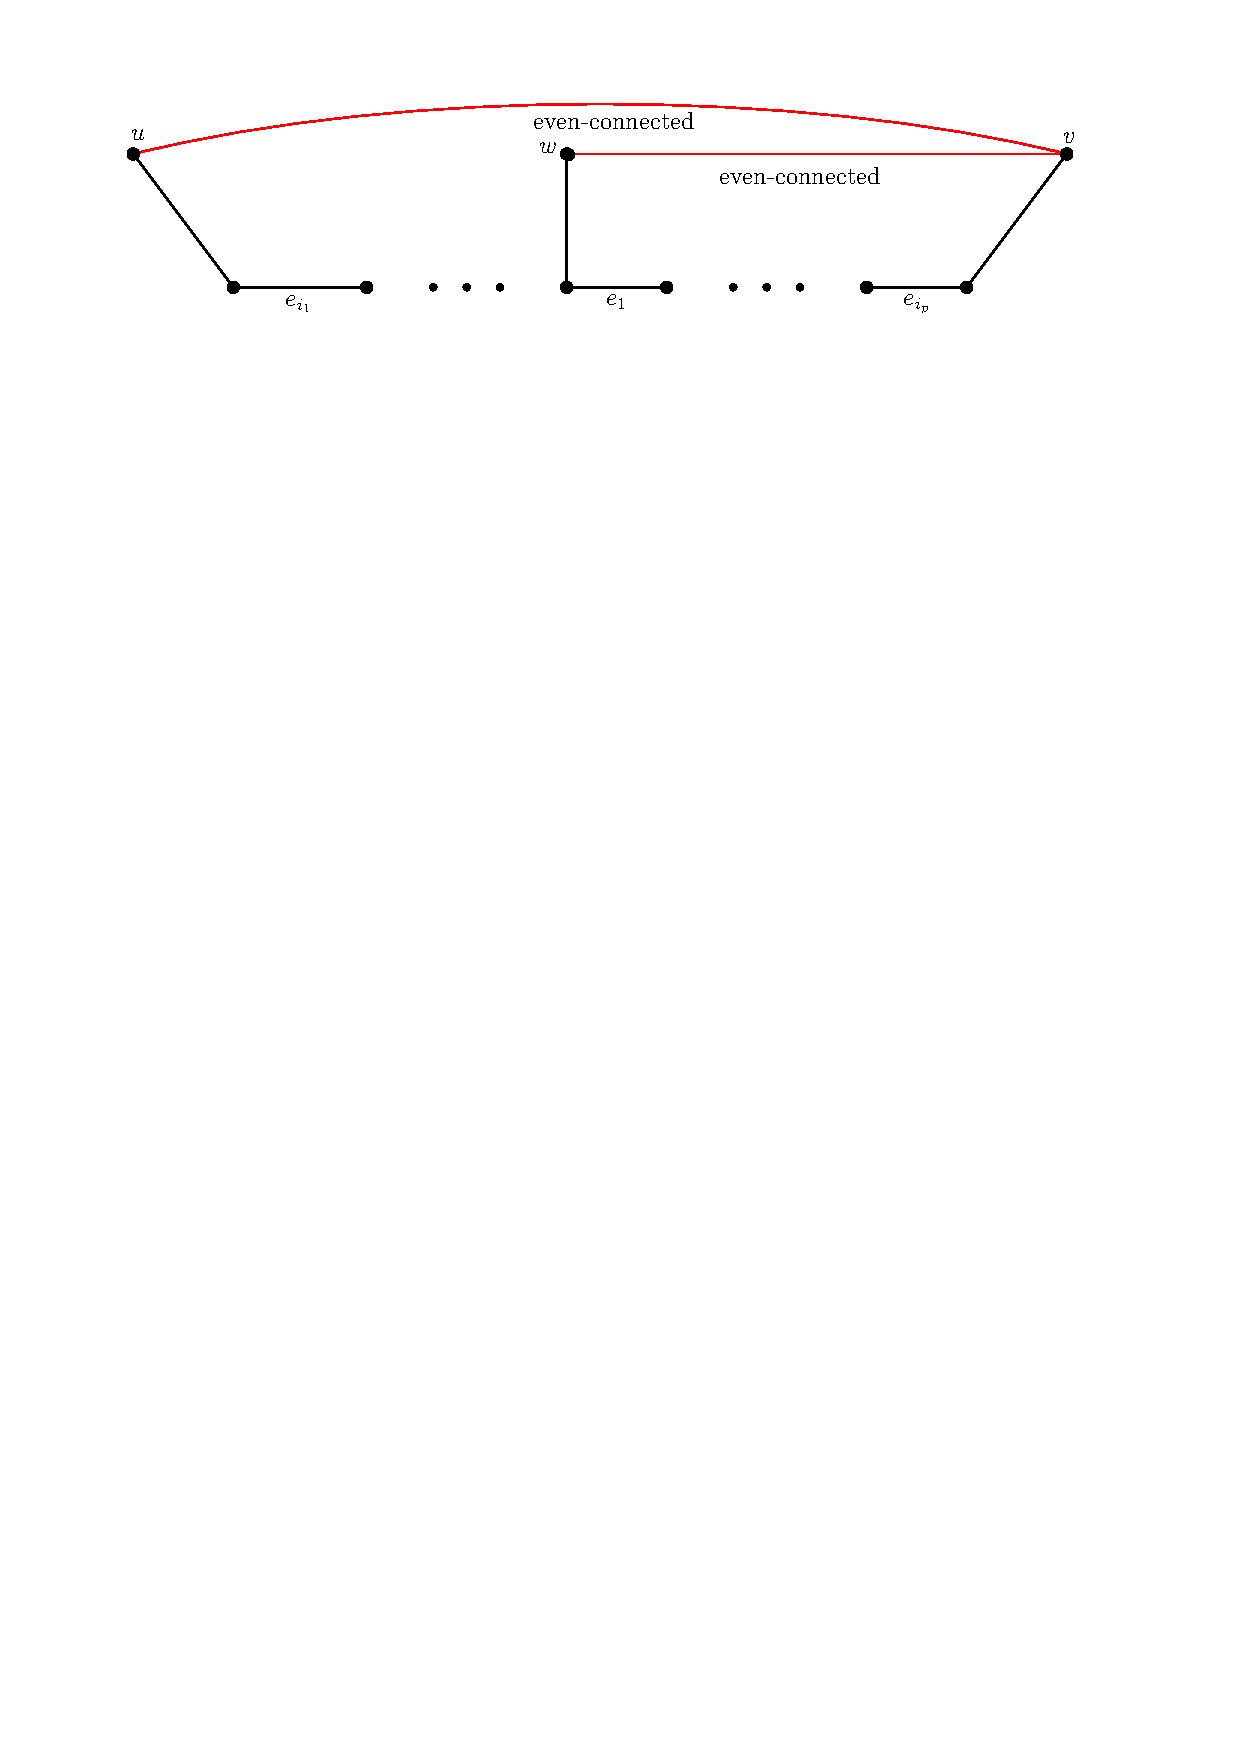
\includegraphics[width=0.9\linewidth]{figures/even2.pdf}
 \caption{When $w \in N_G(e_1)$}
 \label{fig:even2}
\end{figure}

\eqref{lemma3.1_3}~By the definition of even-connection, we first observe that for any subcollection $\{f_1, \dots, f_{t-1}\}$ of $\{e_1, \dots, e_{s-1}\}$ (for some $t \le s$), if $x$ and $y$ are even-connected with respect to $f_1 \cdots f_{t-1}$ in an induced subgraph of $G$ then $x$ and $y$ are also even-connected with respect to $e_1 \cdots e_{s-1}$ in $G$. Thus,
\[
I(G - N_{G'}[w])^t : f_1 \cdots f_{t-1} \subseteq J \subseteq (J:w).
\]

Moreover, for any $u \in N_{G'}(w)$, $u$ and $w$ are even-connected with respect to $e_1 \cdots e_{s-1}$, and so $uw \in J$, \ie $u \in (J : w)$. Thus, we have the inclusion
\[
(I(G - N_{G'}[w])^t : f_1 \cdots f_{t-1}) + (u ~\big|~ u \in N_{G'}(w)) \subseteq (J:w).
\]


To prove the other inclusion, let us analyse the minimal generators of $(J:w)$ more closely. Consider any $uv \in J$, where $u$ and $v$ are even-connected with respect to $e_1 \cdots e_{s-1}$. If $v \equiv w$ (similarly if $u \equiv w$) then $u \in N_{G'}(w)$. If $u,v \not\equiv w$, but $v \in N_{G'}(w)$ (similarly if $u \in N_{G'}(w)$), then $uv$ is subsumed in the ideal $(u ~\big|~ u \in N_{G'}(w))$.

Suppose now that $u,v \not\in N_{G'}[w]$. Then $u,v \in G - N_{G'}[w]$, which are even-connected with respect to $e_1 \cdots e_{s-1}$. Observe that if the even-connected path between $u$ and $v$ contains $e_1$ then, by considering a subpath of this path, either $u$ and $w$ or $v$ and $w$ are even-connected with respect to $e_1 \cdots e_{s-1}$ (see Figures~\ref{fig:even1} and~\ref{fig:even2}). That is, either $u$ or $v$ is in $N_{G'}(w)$, and so $uv$ is again subsumed in the ideal $(u ~\big|~ u \in N_{G'}(w))$. Therefore, we may assume that $u$ and $v$ are even-connected with respect to a subcollection $\{f_1, \dots, f_{t-1}\}$ of $\{e_2, \dots, e_{s-1}\}$. That is, $uv \in I(G - N_{G'}[w])^t : f_1 \dots f_{t-1}$.

\begin{figure}[htb]
 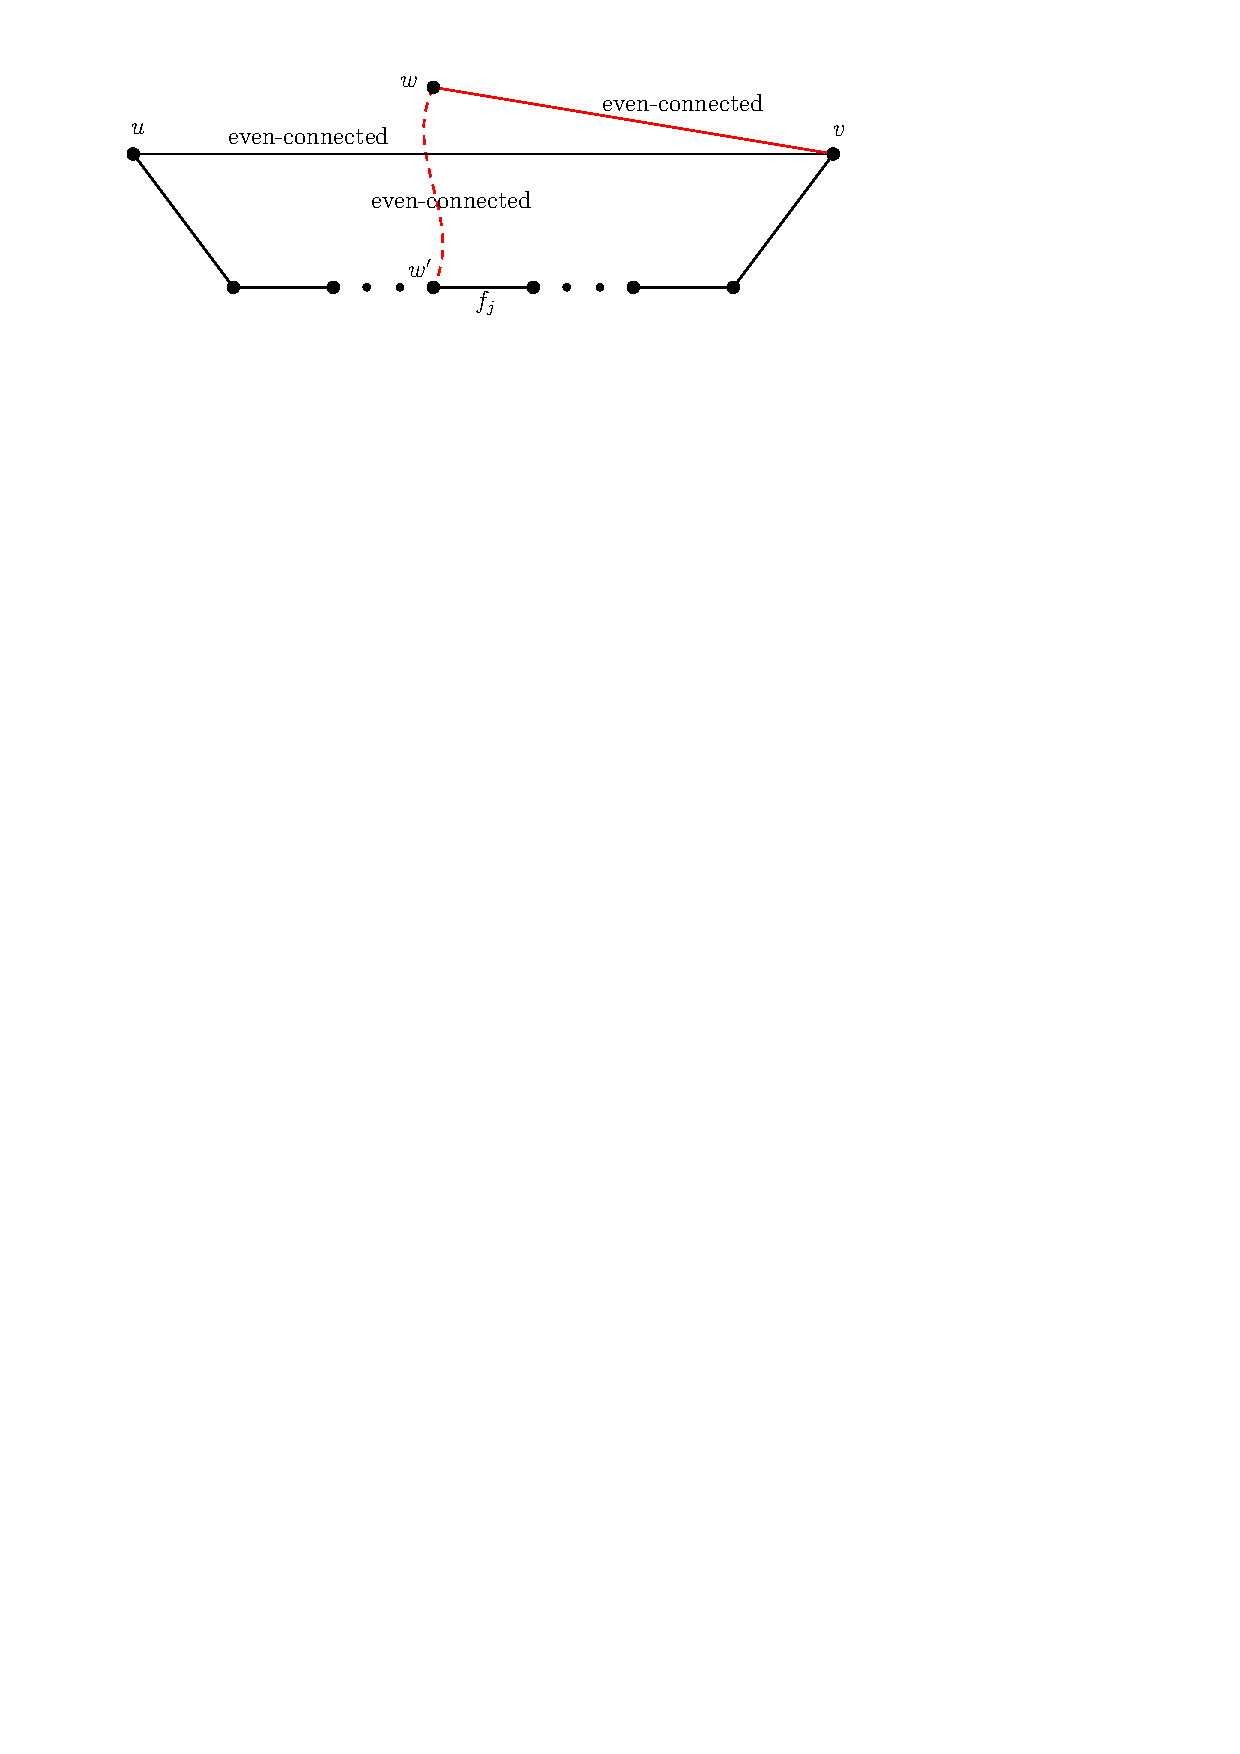
\includegraphics[width=0.7\linewidth]{figures/evenwsub.pdf}
 \caption{When an even-connected path $u$ --- $v$ contains $w' \in N_{G'}[w]$}
 \label{fig:evenwsub}
\end{figure}

To establish the last statement, consider any two vertices $u$ and $v$ which are even-connected in $G-N_G[w]$ with respect to $f_1 \cdots f_{t-1}$. If the even-connected path between $u$ and $v$ does not contain any vertex in $N_{G'}[w] \setminus N_G[w]$ then $u$ and $v$ are even-connected in $G-N_{G'}[w]$. If the even-connected path between $u$ and $v$ contain a vertex $w' \in N_{G'}[w] \setminus N_G[w]$ (see Figure~\ref{fig:evenwsub}) then, by combining with the even-connected path from $w$ to $w'$, either $u$ and $w$ or $v$ and $w$ are even-connected in $G'$. That is, either $u$ or $v$ is already in $N_{G'}[w]$ (or equivalently, not in $G-N_{G'}[w]$). Hence, the graph associated to the polarization of $I(G-N_{G'}[w])^t : f_1 \cdots f_{t-1}$ is an induced subgraph of that associated to the polarization of $I(G-N_G[w])^t : f_1 \cdots f_{t-1}$.
\end{proof}

By understanding local properties of $J$ in Lemma~\ref{lem.induction}, we are able to give a general upper bound for the regularity function based on a well chosen numerical function on families of graphs. Specific interesting general bounds can be obtained by picking these numerical functions suitably.

\begin{defi}
A collection $\F$ of graphs is a \emph{hierarchy} if for every nonempty graph $G \in \F$, both $G - u$ and $G - N_G[u]$ are in $\F$ for any vertex $u \in V(G)$. A nonempty graph is a graph with at least one edge.
\end{defi}
\begin{theo} \label{thm.hierarchy}
Let $\F$ be a hierarchy of graphs. Let $f : \F \longrightarrow \NN$ be a function satisfying the following properties:
\begin{enumerate}
\item\label{theo3.3_1} for any $G \in \F$, $\reg I(G) \le f(G)$; and
\item\label{theo3.3_2} for any nonempty graph $G \in \F$ and each non-isolated vertex $w \in V(G)$,
 \[
f(G-w) \le f(G) \text{ and } f(G - N_G[w]) \le \max\{f(G)-1, 2\}.
\]

\end{enumerate}
Then, for any $G \in \F$ and any $s \ge 1$, we have
\[
\reg I(G)^s \le 2s + f(G) - 2.
\]

\end{theo}
\begin{proof} Fix a graph $G \in \F.$ If $f(G) \le 2$ then $I(G)$ has a linear resolution, and so the result is immediate from~\cite[Theorem 3.2]{HHZ}. Assume that $f(G) \ge 3$. Then the condition on $f(G - N_G[w])$ reads $f(G-N_G[w]) \le f(G)-1.$

By Theorem~\ref{thm.inductive} and the hypothesis that $\reg I(G) \le f(G)$, it suffices to show that for any collection of edges $e_1, \dots, e_{s-1}$ in $G$ (not necessarily distinct), we have
\begin{align}
\reg (I^s : e_1 \cdots e_{s-1}) \le f(G). \label{eq.bounds}
\end{align}
We shall prove~\eqref{eq.bounds} by induction on $s$ and on the size of the graph $G$. Let $J = I^s : e_1 \cdots e_{s-1}$. The statement is trivial if $s = 1$ (whence, $J = I$) or if $G$ is an empty graph (whence, $J = (0)$). Suppose that $s \ge 2$ and $G$ is not an empty graph.

Let $w \in V(G)$ be any vertex in $G$. It follows from Lemma~\ref{lem.induction} that $\reg (J:w)$ is equal to either $\reg (I(G - N_G[w])^s : e_1 \cdots e_{s-1})$ or $\reg (I(G - N_{G'}[w])^t : f_1 \cdots f_{t-1})$ where the graph associated to the polarization of $I(G-N_{G'}[w])^t : f_1 \cdots f_{t-1}$ is an induced subgraph of that associated to the polarization of $I(G-N_G[w])^t : f_1 \cdots f_{t-1}$. If the latter is the case, then by Lemma~\ref{lem.indsubgraph} and the fact that polarization does not change the regularity~\cite[Corollary 1.6.3]{HH}, we have 
\[
\reg (J:w) \le \reg (I(G-N_G[w])^t : f_1 \cdots f_{t-1}).
\]
Thus, since $G-N_G[w] \in \F$, by induction on the size of the graphs and our assumption, we have
\begin{equation}\label{eq:colon}
\reg (J:w) \le f(G-N_G[w]) \le f(G)-1 \text{ for any vertex } w \in V(G).
\end{equation}

By taking, for example, a vertex cover of the graph associated to the polarization of $J$, we may assume that we have a collection of distinct vertices $w_1, \dots, w_l$ of $G$ such that $(J,w_1, \dots, w_l) = (w_1, \dots, w_l)$.

Observe that for each $i = 1, \dots, l-1$, we have
\[
(J,w_1, \dots, w_i):w_{i+1} = (J:w_{i+1}) + (w_1, \dots, w_{i}).
\]
Thus, by~\cite[Corollary 3.2]{Herzog} and~\eqref{eq:colon}, we get
\[
\reg [(J,w_1, \dots, w_i):w_{i+1}] \le \reg (J:w_{i+1}) \le f(G)-1.
\]

This, by successively applying Lemma~\ref{exact} with $(J, w_1, \dots, w_i)$ and $w_{i+1}$, implies that
\[
\reg (J,w_1) \le f(G).
\]
The assertion now follows by utilizing Lemma~\ref{exact} with $J$ and $w_1$.
\end{proof}
\begin{thebibliography}{99}
\bibitem[4]{Ba} Banerjee, Arindam The regularity of powers of edge ideals, J. Algebraic Combin., Volume 41 (2015) no. 2, pp. 303-321.
\bibitem[7]{BrHe} Bruns, Winfried; Herzog, Jürgen Cohen–Macaulay rings, Cambridge university press, 1998 no. 39.
\bibitem[11]{DHS} Dao, Hailong; Huneke, Craig; Schweig, Jay Bounds on the regularity and projective dimension of ideals associated to graphs, J. Algebraic Combin., Volume 38 (2013) no. 1, pp. 37-55.
\bibitem[12]{E} Eisenbud, David Commutative algebra. With a view toward algebraic geometry, Graduate Texts in Mathematics, 150, Springer-Verlag, New York, 1995, xvi+785 pages.
\bibitem[15]{Fr} Fröberg, Ralf On Stanley-Reisner rings, Topics in algebra, Part 2 (Warsaw, 1988) (Banach Center Publ.), Volume 26, PWN, Warsaw, 1990, pp. 57-70.
\bibitem[17]{Harary} Harary, Frank Graph theory, Addison-Wesley Publishing Co., Reading, Mass.-Menlo Park, Calif.-London, 1969, ix+274 pages.
\bibitem[18]{Herzog} Herzog, Jürgen A generalization of the Taylor complex construction, Comm. Algebra, Volume 35 (2007) no. 5, pp. 1747-1756.
\bibitem[19]{HH} Herzog, Jürgen; Hibi, Takayuki Monomial ideals, Graduate Texts in Mathematics, 260, Springer-Verlag London, Ltd., London, 2011.
\bibitem[20]{HHZ} Herzog, Jürgen; Hibi, Takayuki; Zheng, Xinxian Monomial ideals whose powers have a linear resolution, Math. Scand., Volume 95 (2004) no. 1, pp. 23-32.
\bibitem[22]{Hochster} Hochster, Melvin Cohen–Macaulay rings, combinatorics, and simplicial complexes, Ring theory, II (Proc. Second Conf., Univ. Oklahoma, Norman, Okla., 1975) (Lecture Notes in Pure and Appl. Math.), Volume 26 (1977), pp. 171-223.
\bibitem[27]{L} Lyubeznik, Gennady The minimal non-Cohen–Macaulay monomial ideals, J. Pure Appl. Algebra, Volume 51 (1988) no. 3, pp. 261-266.
\bibitem[28]{MS} Miller, Ezra; Sturmfels, Bernd Combinatorial commutative algebra, Graduate Texts in Mathematics, 227, Springer Science \& Business Media, 2004.
\bibitem[33]{Stanley} Stanley, Richard P. Combinatorics and commutative algebra, Progress in Mathematics, 41, Birkhäuser, 2007.
\bibitem[36]{V} Villarreal, Rafael Monomial algebras, CRC Press, 2018.
\bibitem[37]{Wegner} Wegner, Gerd d-collapsing and nerves of families of convex sets, Arch. Math. (Basel), Volume 26 (1975), pp. 317-321.
\end{thebibliography}
\end{document}
